\documentclass[12pt]{article}
\usepackage[margin=0.7in]{geometry} 		% defines page margin
\usepackage{knitting} 				% defines \chart and \textknit
\usepackage{titling} 				% title page
\usepackage{graphicx,xspace, scrextend}	% defines space control stuff
\usepackage{tabularx, array, colortbl}	% defines tables
\usepackage{multicol} 				% defines columns
\usepackage{multirow} 				% defines multirows, combined cells in tables
\usepackage{framed} 				% defines boxes for notes and written directions
\usepackage[x11names]{xcolor} 		% extends color library
\pdfmapfile{+knitfont.map}

\renewcommand{\arraystretch}{2}

\newcolumntype{L}[1]{>{\leftalign\arraybackslash}p{#1}}
\newcolumntype{C}[1]{>{\centering\arraybackslash}p{#1}}

% length parameters
\setlength{\parindent}{0pt} % disables indentation for paragraphs
\setlength{\columnsep}{0.7cm} % column separation in multicol environment

% color parameters
\colorlet{framecolor}{black}
\colorlet{shadecolor}{LemonChiffon1}
\colorlet{highlight}{yellow}

% custom commands
\newcommand{\comment}[1]{} % allows for multiline comments that LaTeX will ignore

\newcommand{\vocab}[1]{\emph{\textbf{#1}}} % format for highlighting definitions of stitches, vocabulary terms
\newcommand{\rowDir}[1]{\textbf{#1:}} % indent for written instructions within paragraphs

\renewcommand{\repeat}[1]{\textbf{*[#1]*}} % format for written repeats, bold with *[ stitches ]*

\newcommand{\increase}[1]{(\emph{+#1 
	\ifnum#1=1{st}\else{sts}\fi})}
\newcommand{\decrease}[1]{(\emph{$-$#1
	\ifnum#1=1{st}\else{sts}\fi})}
\newcommand{\stitchcount}[1]{(\emph{#1 sts})}

\renewcommand{\rm}{\emph{rm}} % remove marker
\renewcommand{\pm}{\emph{pm}} % place marker

% thick horizontal line
\makeatletter \newcommand{\thickhline}{
    \noalign {\ifnum 0=`}\fi \hrule height 1.5pt
    \futurelet \reserved@a \@xhline
}
\makeatother

% custom environments
\newenvironment{frnote}
    {% framed environment for pattern notes
    	\setlength{\FrameRule}{1.5pt}
    	\def\FrameCommand{\fboxrule=\FrameRule\fboxsep=\FrameSep \fcolorbox{framecolor}{shadecolor}}
    	\MakeFramed {\FrameRestore}}
    {\setlength{\FrameRule}{1pt}
	\endMakeFramed}

\newenvironment{frdirection}
    {% framed environment for written directions
	\def\FrameCommand{\fboxrule=\FrameRule\fboxsep=\FrameSep \fbox}
   	\MakeFramed {\advance\hsize-\width \FrameRestore}
    	\addmargin[1.5cm]{0pt}}
    {\endaddmargin
	\endMakeFramed}

\newenvironment{unframed}
    {% unframed environment for written directions
	\begin{addmargin}[2em]{0pt}
	\setlength{\parindent}{-2em}}
    {\vspace{1em}
	\setlength{\parindent}{0em}
	\end{addmargin}}

\title{Pops and Pins}
\author{Shanel Wu (Piper Nell)}

\begin{document}
\begin{titlingpage}

\begin{multicols}{2}
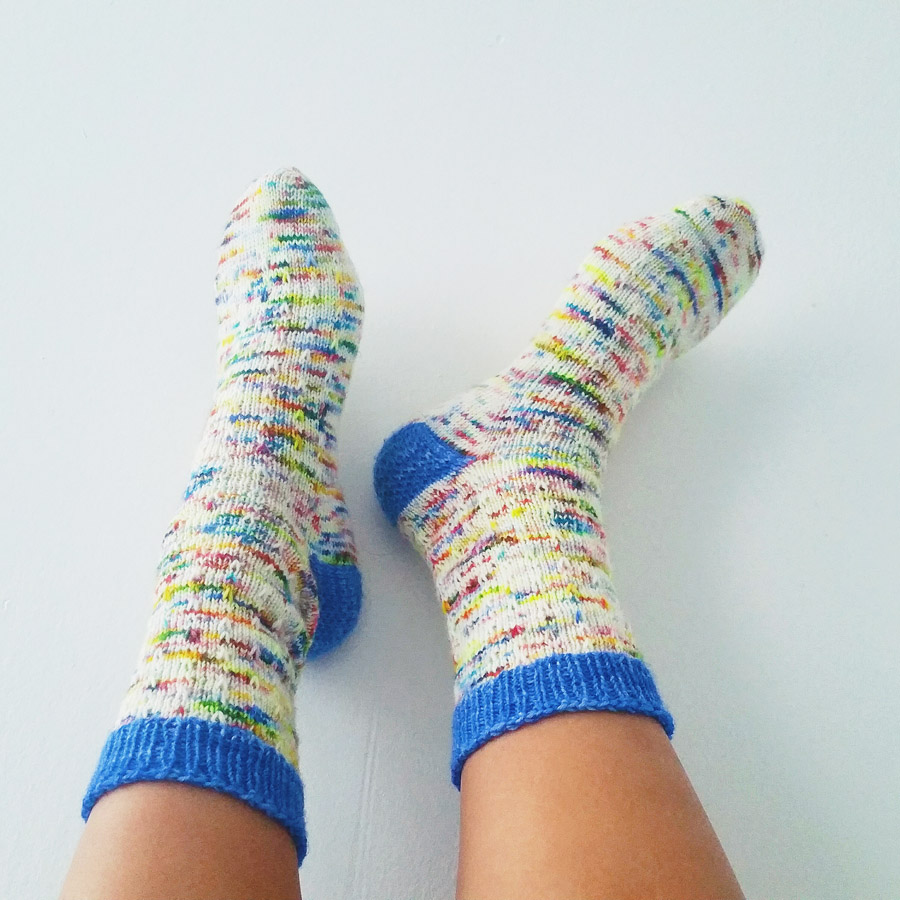
\includegraphics[height=3.5in]{feetWall.jpg}

\vfill

\section*{\thetitle}
\vspace{-0.5em}
\subsubsection*{\theauthor}

Grab a skein of speckled yarn and watch the colors \emph{pop} in a slip-stitch \emph{pins} texture!

\vspace{-1em}
\subsubsection*{Materials}

\begin{itemize}
\item 100g fingering weight sock yarn in MC
\item 20g sock yarn in CC (optional)
\item Long circular needle for Magic Loop (your preferred size for gauge)
\end{itemize}

Although the pattern calls for Magic Loop, it can be adapted for 2 circs or 4 DPN's.

\vspace{-1em}
\subsubsection*{Gauge/Sizing}

This pattern is written for two sock gauges: \vocab{S} (56 sts) and \vocab{M} (64 sts.) The sample was knitted on 64sts with US1/2.25mm needles. To size up or down, either adjust needle size or stitch count.

\subsubsection*{Techniques}

This sock pattern is written for intermediate sock knitters. Prior to beginning this pattern, you'll need to know basic toe-up sock construction, Judy's Magic Cast On, simple increases and decreases, short rows, and slipping stitches.

\vfill 
\columnbreak

\small 			% FONT SIZE CHANGE
\subsection*{Pattern Key}
Stitch counts and repeats will be given as \vocab{S (M)} [e.g. 28(32) sts]. Pattern repeats will be indicated with thick borders (chart) or \textbf{*[stitches]*} (written).

\vspace{-1em}

\begin{center}
\begin{tabular}{| C{0.12\linewidth}  C{0.2\linewidth}  p{0.55\linewidth} | }
\thickhline \rowcolor{shadecolor} 
\textbf{Chart}	& \textbf{Written}	& \textbf{Name \& Description} \\ \thickhline
\chart{-}	& k	&  knit	\\
\chart{v}	& s1		& \textbf{slip 1} stitch purlwise with yarn in back (wyib) \\
\chart{z}	& w2k		& \textbf{wrap 2 knit:} insert needle into stitch as if to knit, wrap yarn twice and pull both loops through; produces doubled stitch \\
\chart{Y}	& s1dl		& \textbf{slip 1 drop loop:} slip doubled stitch wyib, drop second wrap \\ \hline
\end{tabular}

\vspace{1em}

\begin{tabular}{| C{0.2\linewidth} p{0.72\linewidth} |}
\thickhline \rowcolor{shadecolor} 
\textbf{Written}	& \textbf{Name \& Description} \\ \thickhline
ssp	& \textbf{slip slip purl:} s1 knitwise, s1 knitwise, sl2 back to left needle, p2tog tbl \\
kfb	& \textbf{knit front back:} knit stitch through front loop as usual, then in the same stitch, knit through the back loop; single increase \\
m1l 		& \textbf{make 1 left:} with right needle, pick up bar between sts back to front, knit tbl; single increase, left-leaning \\
m1r 		& \textbf{make 1 right:} pick up bar between sts front to back, knit through front loop; single increase, right-leaning \\
m1p 		& \textbf{make 1 purlwise:} wyif, pick up bar between sts back to front, purl tbl; single increase, left-leaning \\
w\&t 		& \textbf{wrap \& turn:} s1 wyib, bring yarn to front, s1 back to left needle to ``wrap" stitch, turn \\ \hline
\end{tabular}
\end{center}
\end{multicols}
\normalsize

\end{titlingpage}

\begin{multicols}{2}
%%%%%%%%%%%%%%%%%%%%%%%%%%%%%%%%%%%%%%%%%%%
\subsection*{Rounded Toe Increases}

With CC, CO 20 sts using Judy's Magic Cast On. Knit all stitches for one round, then work toe increases through Round 16 (Round 24) until stitch count is 56 (64) sts.
\begin{unframed}
\hspace{-2em}\rowDir{Rnd 1 (increase round)} k1, m1l, k to last 1 st on needle, m1r, k1, repeat on needle 2. \stitchcount{24}

\rowDir{Rnd 2} Increase round. \stitchcount{28}

\rowDir{Rnd 3} Increase round. \stitchcount{32}

\rowDir{Rnd 4} Increase round. \stitchcount{36}

\rowDir{Rnd 5} Increase round. \stitchcount{40}

\rowDir{Rnd 6} k across.

\rowDir{Rnds 7-8} Repeat Rnds 5-6. \stitchcount{44}

\rowDir{Rnds 9-10} Repeat Rnds 5-6. \stitchcount{48}

\rowDir{Rnds 11-12} Repeat Rnds 5-6. \stitchcount{52}

\rowDir{Rnd 13} Increase round. \stitchcount{56}

\rowDir{Rnds 14-16} k across.

\rowDir{Rnds 17-20} Repeat Rnds 13-16. \stitchcount{60}

\rowDir{Rnds 21-24} Repeat Rnds 13-16. \stitchcount{64}
\end{unframed}

Switch to MC. Your ``instep stitches" are now on needle 1 and your ``sole stitches" are on needle 2. You should have 28 (32) sts on each needle.

\small
\subsection*{Pops and Pins (chart)}

\chart{
\!\overline{--------}\! \rnright
\!-v------\! \rnright
\!-Y---v--\! \rnright
\!-z------\! \rnright
\!--------\! \rnright
\!-----v--\! \rnright
\!-v---Y--\!\rnright
\!\underline{-----z--}\! \rnright
}

\subsection*{Pops and Pins (written)}

\rowDir{Rnd 1} k2, \repeat{w2k, k7}, w2k, k5

\rowDir{Rnd 2} k2, \repeat{s1dl, k3, s1, k3}, s1dl, k3, s1, k1

\rowDir{Rnd 3} k2, \repeat{s1, k7}, s1, k5

\rowDir{Rnd 4} k across

\rowDir{Rnd 5} k6, \repeat{w2k, k7}, w2k, k1

\rowDir{Rnd 6} k2, s1dl, k3, \repeat{s1dl, k3, s1, k3}, s1dl, k1

\rowDir{Rnd 7} k6, \repeat{s1, k7}, s1, k1

\rowDir{Rnd 8} k across

\normalsize
\subsection*{Foot}

Work ``Pops and Pins" stitch repeat 3.5 (4) times across the instep. For a 56 st sock, work 3 repeats then the first 4 sts of the pattern. Work sole stitches in stockinette. Repeat stitch pattern until foot is 3 inches shorter than desired foot length.

\vspace{-1em}
\begin{flushright}
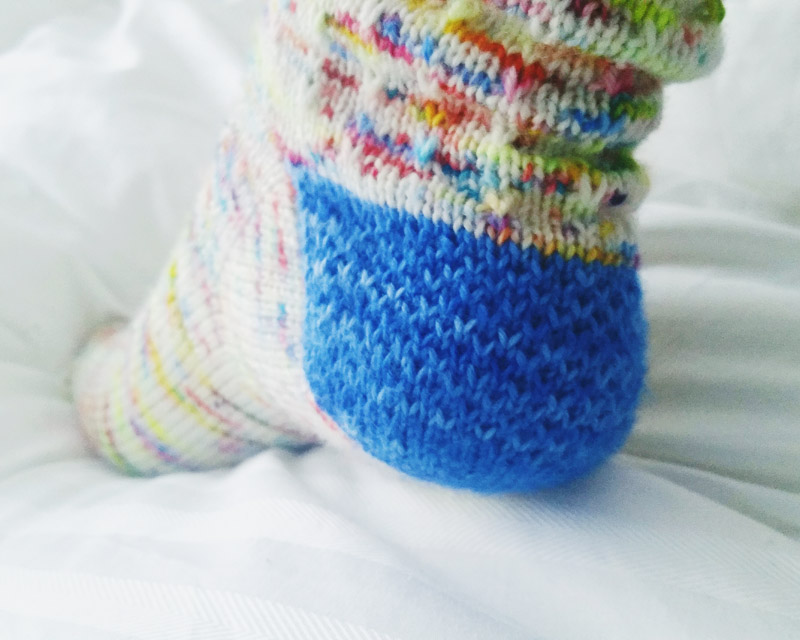
\includegraphics[height=1.7in]{heel.jpg}
\end{flushright}

\vspace{-4em}

\subsection*{Heel$*$}
Continue working across instep in established pattern without changing stitch count. Your sole stitches will now become the ``heel stitches" and you will increase on the heel needle to form the gusset.
\vspace{-1em}
\subsubsection*{Gusset Increases}
\vspace{-0.5em}
\begin{unframed}
\hspace{-2em}\rowDir{Rnd 1} Work across instep. On heel needle, k1, m1l, k to last st, m1r, k1. \increase{2}

\rowDir{Rnd 2} Work across instep. K across heel.
\end{unframed}

Work a total of 10 repeats of the 2 gusset increase rounds until you have 48 (52) heel sts \\{} [76 (84) sts total].

\vspace{-.5em}
\subsubsection*{Heel Turn}
\vspace{-.5em}
Work across instep. For contrasting heels, \vocab{switch to CC --  DO NOT cut MC.} Work back and forth on the heel needle as follows:
\begin{unframed}
\hspace{-2em}\rowDir{Row 1} (RS) k 32 (34) to last 16 (18) sts, \\ m1r, k1, w\&t

\rowDir{Row 2} (WS) p18 to last 16 (18) sts, \\ m1p, p1, w\&t

\rowDir{Row 3} k16, m1r, k1, w\&t

\rowDir{Row 4} p14, m1p, p1, w\&t

\rowDir{Row 5} k12, m1r, k1, w\&t

\rowDir{Row 6} p10, m1p, p1, w\&t

\rowDir{Row 7} k8, m1r, k1, w\&t

\rowDir{Row 8} p6, m1p, p1, w\&t
\end{unframed}
\increase{8} in total. You should have 56 (60) sts heel sts after the heel turn.

\newpage
\begin{frnote}
\vocab{Picking Up Wraps}
\vspace{.5em}

\textbf{RS:} With right needle, pick up front leg of wrap by inserting needle front to back. Insert needle knitwise into wrapped st, then knit together. 

\textbf{WS:} Pick up back leg of wrap by inserting needle back to front. Insert needle purlwise into wrapped st, then purl together.
\end{frnote}

Work the following two ``boomerang" rows to complete the heel turn and begin the heel flap:

\rowDir{Boomerang 1} (RS) k across the heel to 1 st from end, picking up wraps and knitting them together with their sts as they come. At the last heel stitch, w\&t.

\rowDir{Boomerang 2} (WS) s1, p across to 1 st from end, picking up wraps and purling them together with their sts as they come. At the last st, w\&t.

\subsubsection*{Heel ``Flap"}
\vspace{-.5em}
Now you will finish the heel by joining the gusset stitches to a heel ``flap" (which never actually flaps around) that is worked back and forth. You should have 1 st on the R needle to start. 

\rowDir{Set Up 1} (RS) k 40 (44) to 15 sts from end, ssk and turn. \emph{(creates first gap)}

\rowDir{Set Up 2} (WS) s1, p 26 (30) to 15 sts from end, p2tog and turn. \emph{(creates second gap)}

\vspace{1em}
After the set up rows, your heel stitches should look like: \vocab{(left to right)} 13 sts, first gap, 28 (32) sts, second gap, 13 sts -- total of 54 (58) sts. 

Repeat the following 4 rows until you have 30 (34) heel sts, then follow the directions given for the last 2 decreases.

\rowDir{Row 1} (RS) s1, \repeat{k1, s1} to 1 st before the first gap, ssk and turn. \decrease{1}

\rowDir{Row 2} (WS) s1, p 26 (30) to 1 st before the second gap, p2tog and turn. \decrease{1}

\rowDir{Row 3} (RS) s1, \repeat{s1, k1} to 1 st before the first gap, ssk and turn. \decrease{1}

\rowDir{Row 4} (WS) Repeat Row 2. \decrease{1}


\vspace{1em}
\rowDir{Last RS decrease} s1, k 26 (30) to 1 before the gap, s1, pick up wrap and knit together, pass slipped st over, and turn. 

\rowDir{Last WS decrease} s1,  p 26 (30) to 1 before the gap, s1, pick up wrap and purl together, psso, and turn.

\vfill
\columnbreak
You should be back to 28 (32) heel sts. For contrasting heels, \vocab{switch back to MC}.


\subsection*{Leg}
Work 7 (8) repeats of the ``Pops and Pins" stitch pattern on front and back of sock until leg is desired length.
\vspace{-1em}
 

\subsubsection*{Transition to Cuff (optional)} 
\vspace{-.5em}
To create a scalloped transition to the contrasting cuff, work Round 1 of ``Pops and Pins" once more. \vocab{Switch to CC}. Work the following transition rounds:
\small
\begin{unframed}
\hspace{-2em}\rowDir{Rnd 1} \repeat{k1, p1, sldl, p1, k1, p1, s1, p1}

\rowDir{Rnd 2} \repeat{k1, p1, s1, p1, k1, p1, k1, p1}
\end{unframed}
\normalsize
\vspace{-1em}

\subsection*{Cuff and Finishing}

Work 1x1 ribbing: \repeat{k1, p1} until cuff is desired length. Bind off loosely with a stretchy BO (I recommend a sewn bind-off or JSSBO).

\vfill

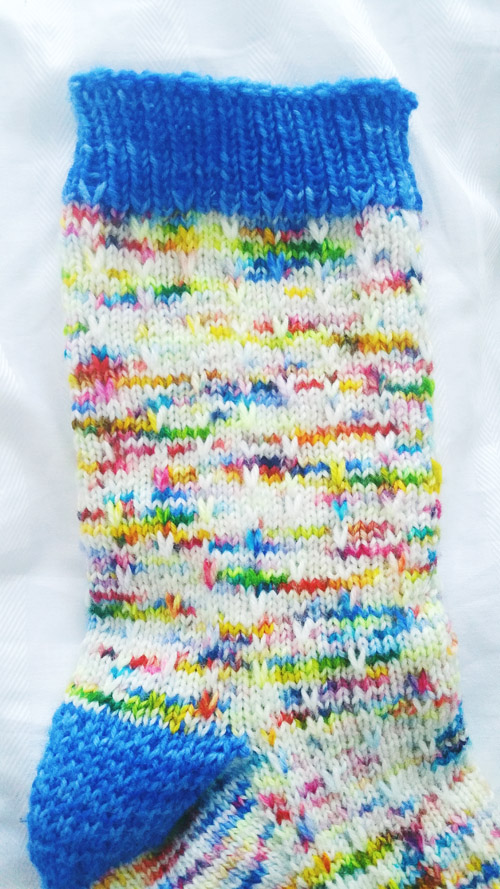
\includegraphics[width=2.3in]{detail.jpg}

\vfill

\small
$*$ \emph{This heel method heavily references the ``Generic Toe-Up, Slip-Stitch Heel, Sock Formula" by Sarah Keller, available as a free pattern on Ravelry.} \\  http://www.ravelry.com/patterns/library/generic-toe-up-slip-stitch-heel-sock-formula
\end{multicols}


\end{document}